\section{Spezifikation der Inventursoftware} \label{software}

Um die Bilddaten der Drohne für eine Inventur zu verarbeiten, soll die Drohne von einer Client-Anwendung angesprochen werden. Der Server, der als Client agiert und im \textit{Flask} Framework für Python zu schreiben ist, soll sich zur Drohne verbinden und die Flugsignale als Fluganweisungen zur Drohne senden. Da die Drohne keinerlei Sensoren zur Detektion möglicher Hindernisse enthält und es zudem nicht das Ziel ist, die Drohne automatisiert fliegen zu lassen, wird die Flugroute statisch als Flugsequenz festgelegt. Die Drohne soll dabei links oben starten und im Uhrzeigersinn die einzelnen Objektgruppen des Regals abfliegen. Dadurch soll eine möglichst genaue Detektion der einzelnen Objekte ermöglicht werden. Zum Schluss soll die Drohne den Blick auf das gesamte Regal ermöglichen und etwas zurück fliegen, damit auch die Detektion aller Objektklassen gemeinsam aus größerer Distanz getestet werden kann.

Auf dem Server soll zudem das \textit{Deep Learning} Modell zur Inferenz integriert werden. Aufgabe des Servers soll es sein, die von der Drohne empfangenen Video-Stream-Frames mit dem Modell zu inferieren, die detektierten Objekte für die Inventur mit Hilfe eines Zählalgorithmus zu zählen und die Bilddaten mit den eingezeichneten Bounding Boxen anschließend per Livestream an eine Webapplikation zur Visualisierung weiterzugeben. Eine \textit{REST} Schnittstelle soll Aussagen über die Bestandsdaten des Warenhauses liefern.

\begin{figure}[ht]
	\begin{center}
		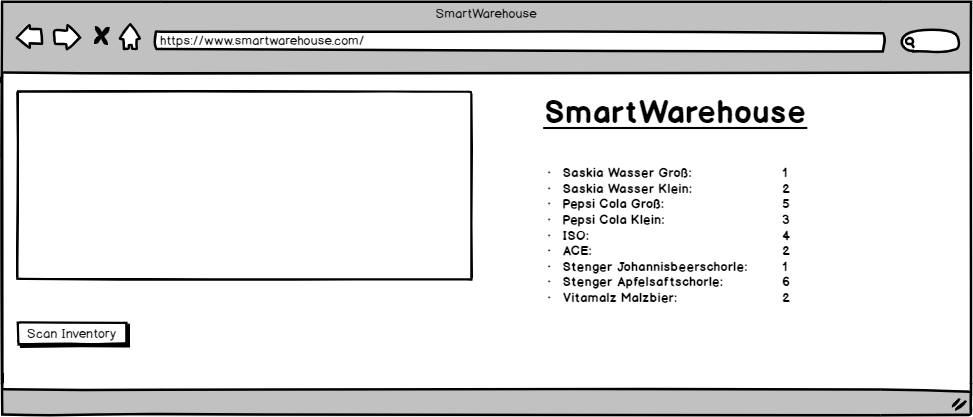
\includegraphics[width=15cm]{Bilder/UI.png} 
		\caption[SmartWarehouse User Interface Prototyp]{SmartWarehouse User Interface Prototyp}
		\label{ui}
	\end{center}
\end{figure}

Die Client-Anwendung soll das Live-Drohnenbild mit den eingezeichneten, erkannten Objekten zeigen. Zudem wird die Anzahl an erkannten Objekten der spezifischen Klassen rechts daneben dargestellt. 
